\documentclass[12pt,letterpaper]{article}
\usepackage[margin=0.65in,top=0.78in,bottom=0.68in,headheight=15pt,headsep=17pt]{geometry}
\usepackage[T1]{fontenc}
\usepackage{helvet}
\renewcommand{\familydefault}{\sfdefault}
\usepackage{tikz}
\usetikzlibrary{arrows.meta}
\usepackage{fancyhdr}
\usepackage{array}
\pagestyle{fancy}
\fancyhf{}
\newcommand{\band}{Grades 3--5}
\fancyhead[L]{\small Week 60 / Take it or pass / \band}
\fancyfoot[L]{\footnotesize Bellingham Math Circle / Week 60 / W60-S-v2}
\fancyfoot[R]{\footnotesize\thepage}
\renewcommand{\headrulewidth}{0.4pt}
\renewcommand{\footrulewidth}{0pt}
\setlength{\parindent}{0pt}
\setlength{\parskip}{7pt}
\setlength{\tabcolsep}{7pt}
\pdfinfoomitdate=1
\pdftrailerid{}
\newcommand{\problem}[2]{\textbf{Problem #1:} #2\par}
\newcommand{\blanklines}[1]{\foreach \i in {1,...,#1}{\par\vspace{0.28in}\noindent\rule{\linewidth}{0.25pt}}}
\newcommand{\cardtwo}[4]{%
  \begin{scope}[shift={({#1},{#2})}]
    \draw[dashed,gray] (0,0) rectangle (2.15,0.88);
    \node[font=\Large] at (0.69,0.59) {#3};
    \node[font=\Large] at (1.46,0.59) {#4};
    \draw[gray] (1.075,0.43) -- (1.075,0.75);
    \node[font=\small] at (1.075,0.20) {score \rule{0.69in}{0.35pt}};
  \end{scope}}
\newcommand{\cardthree}[5]{%
  \begin{scope}[shift={({#1},{#2})}]
    \draw[dashed,gray] (0,0) rectangle (2.15,0.70);
    \node[font=\large] at (0.45,0.47) {#3};
    \node[font=\large] at (1.075,0.47) {#4};
    \node[font=\large] at (1.70,0.47) {#5};
    \draw[gray] (0.76,0.34) -- (0.76,0.60);
    \draw[gray] (1.39,0.34) -- (1.39,0.60);
    \node[font=\small] at (1.075,0.17) {score \rule{0.69in}{0.35pt}};
  \end{scope}}
\newcommand{\position}[2]{%
\begin{tikzpicture}[x=1in,y=1in]
\draw[rounded corners=3pt] (0,0) rectangle (2.85,1.22);
\node[font=\small] at (1.425,0.99) {#2 offers left, including this one};
\draw (0.27,0.24) rectangle (0.85,0.78);
\node[font=\Large] at (0.56,0.51) {#1};
\foreach \i in {1,...,#2}{\draw (1.02+\i*0.38,0.52) circle (0.12);}
\node[font=\small] at (1.94,0.24) {turn counters};
\end{tikzpicture}}
\begin{document}

Each bag has one ticket marked 0, one marked 4 and one marked 6. Each has the same chance. Return the ticket and mix after \emph{every} draw. The next offer is a fresh draw from the same bag.

Set the number of offers before a round. Your partner shows each offer. Take it to end the round, or pass it forever. With one counter left, you must take the offer, even if it is 0. Remove one turn counter after deciding on each offer. Only the offer you take scores.

A practice round uses different tickets: 1, 2, 5.

\begin{center}
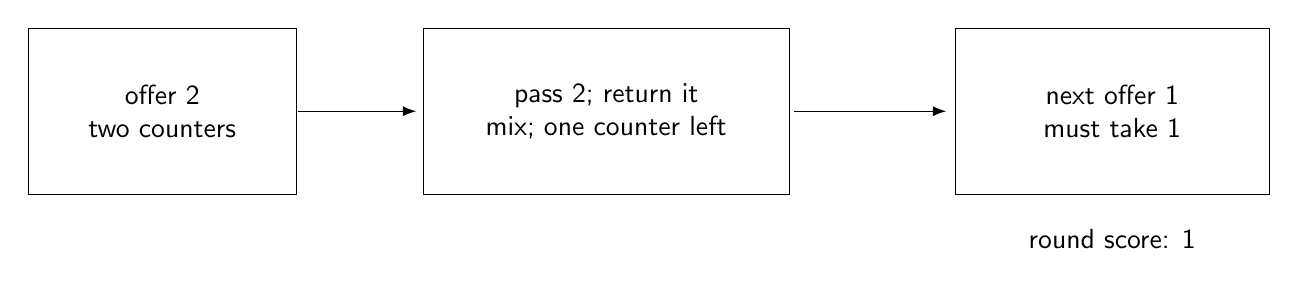
\begin{tikzpicture}[x=1in,y=1in,>=Latex]
  \node[draw,minimum width=1.34in,minimum height=0.83in,align=center] at (0.8,0.45) {offer 2\\two counters};
  \node[draw,minimum width=1.83in,minimum height=0.83in,align=center] at (3.02,0.45) {pass 2; return it\\mix; one counter left};
  \node[draw,minimum width=1.57in,minimum height=0.83in,align=center] at (5.55,0.45) {next offer 1\\must take 1};
  \draw[->] (1.48,0.45) -- (2.07,0.45);
  \draw[->] (3.96,0.45) -- (4.72,0.45);
  \node at (5.55,-0.19) {round score: 1};
\end{tikzpicture}
\end{center}

\problem{1}{Use the 0, 4, 6 bag. Invent a taking rule for two-offer rounds and one for three-offer rounds. Keep each rule fixed while playing six rounds with a partner. Try to get a high total score. Swap roles.}

\vspace{0.08in}
\begin{tabular}{@{}p{1.42in}p{5.33in}@{}}
Two-offer rule & \rule{5.25in}{0.3pt}\\[0.35in]
Three-offer rule & \rule{5.25in}{0.3pt}
\end{tabular}

\vspace{0.27in}
\begin{center}
\renewcommand{\arraystretch}{2.1}
\begin{tabular}{|p{1.48in}|*{6}{p{0.44in}|}p{0.63in}|}
\hline
Round & 1 & 2 & 3 & 4 & 5 & 6 & Total\\\hline
Two offers & & & & & & & \\\hline
Three offers & & & & & & & \\\hline
\end{tabular}
\end{center}

\vspace{0.14in}
\problem{2}{Can the same fixed rules give opposite winners in two six-round matches? Show possible offers for both. Can either match settle which rule has the better average over many rounds?}
\blanklines{3}

\newpage
\renewcommand{\band}{Grades 3--5}
A card lists offers in drawing order, including offers that would remain unseen after you take one. All complete cards of the same length have the same chance.

With practice tickets 1, 3, 5, this rule takes 3 or 5 and passes 1:
\begin{center}
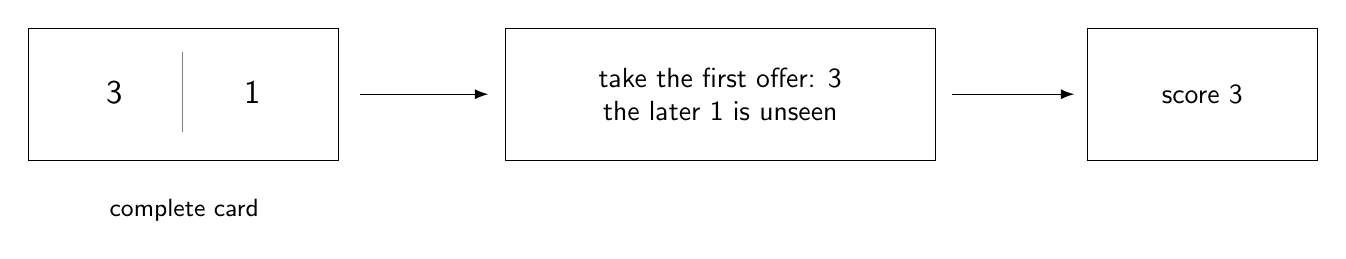
\begin{tikzpicture}[x=1in,y=1in,>=Latex]
  \draw (0,0.06) rectangle (1.55,0.72);
  \node[font=\large] at (0.43,0.40) {3};
  \node[font=\large] at (1.12,0.40) {1};
  \draw[gray] (0.77,0.20) -- (0.77,0.60);
  \node[font=\small] at (0.78,-0.19) {complete card};
  \draw[->] (1.66,0.39) -- (2.30,0.39);
  \node[draw,align=center,minimum width=2.15in,minimum height=0.66in] at (3.46,0.39) {take the first offer: 3\\the later 1 is unseen};
  \draw[->] (4.62,0.39) -- (5.23,0.39);
  \node[draw,minimum width=1.15in,minimum height=0.66in] at (5.87,0.39) {score 3};
\end{tikzpicture}
\end{center}

\problem{3}{Find first-offer choices for 0, 4 and 6 that give the highest total score on all nine cards. Use the same choices on every card. The second offer must be taken if you reach it.}

\begin{center}
\begin{tikzpicture}[x=1in,y=1in]
\foreach \a [count=\r from 0] in {0,4,6}{
\foreach \b [count=\c from 0] in {0,4,6}{
\cardtwo{\c*2.28}{(2-\r)*1.01}{\a}{\b}
}}
\end{tikzpicture}
\end{center}

\vspace{0.15in}
\begin{tabular}{@{}p{2.06in}p{2.06in}p{2.06in}@{}}
First offer 0: & First offer 4: & First offer 6:\\[0.30in]
\rule{1.9in}{0.3pt} & \rule{1.9in}{0.3pt} & \rule{1.9in}{0.3pt}
\end{tabular}

\vspace{0.24in}
Total score on nine cards: \rule{1.55in}{0.3pt}
\blanklines{2}

\newpage
\renewcommand{\band}{Grades 3--5}
\problem{4}{Which plan gives the higher total score on these 27 three-offer cards? Use every card for each plan, including cards with the same score.}

A: Take 4 or 6 whenever it appears. Pass 0.\par
B: Take only 6 on the first offer. On the second, take 4 or 6 and pass 0.\par
Both plans take the last offer if they reach it.

A's total: \rule{1.12in}{0.3pt}\hspace{0.45in}B's total: \rule{1.12in}{0.3pt}

\vspace{-0.02in}
\begin{center}
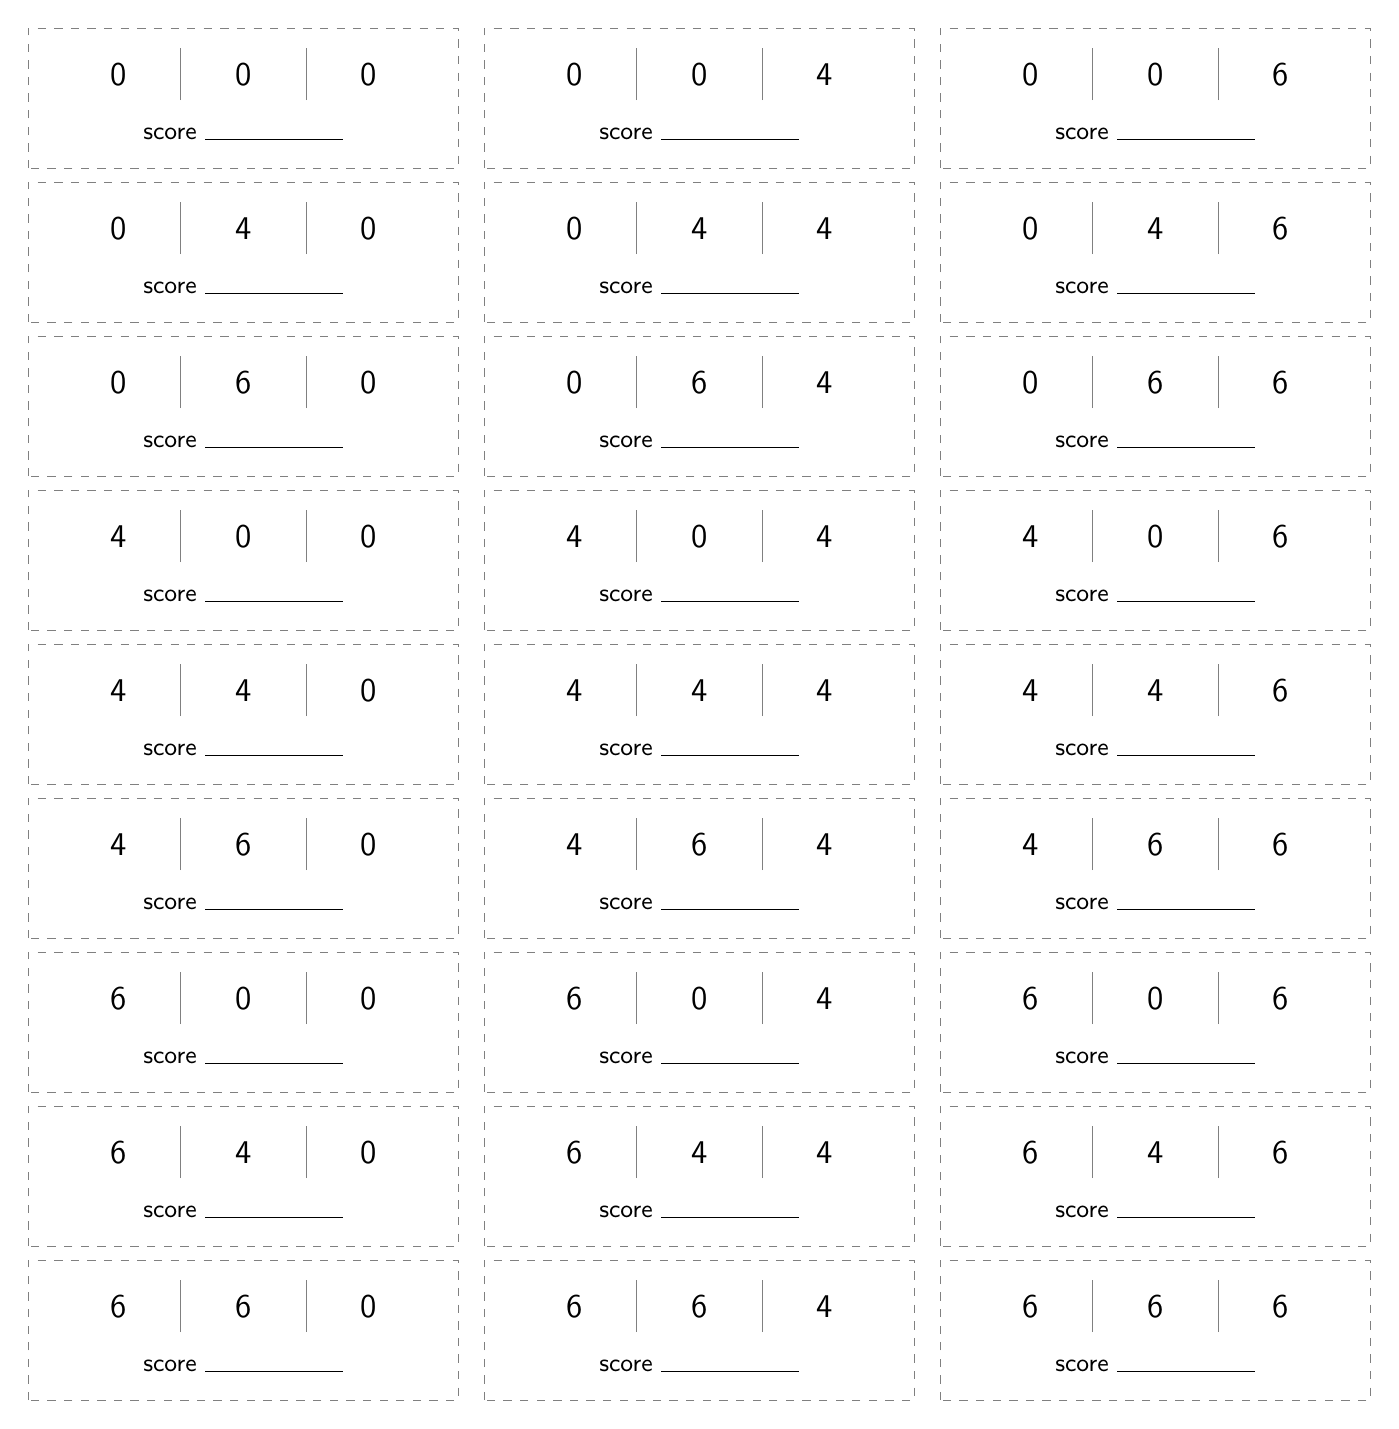
\begin{tikzpicture}[x=1in,y=1in]
\foreach \a [count=\r from 0] in {0,4,6}{
\foreach \b [count=\s from 0] in {0,4,6}{
\foreach \c [count=\t from 0] in {0,4,6}{
\cardthree{\t*2.28}{(8-3*\r-\s)*0.77}{\a}{\b}{\c}
}}}
\end{tikzpicture}
\end{center}

\newpage
\renewcommand{\band}{Grades 4--5}
\problem{5}{The current offer is 4. Compare taking 4 with your best plan after passing 4. Which choice has the higher average score in each position? Use all possible future offers from the 0, 4, 6 bag to support your choices.}

\begin{center}
\position{4}{2}\hspace{0.35in}\position{4}{3}
\end{center}

\begin{minipage}[t]{3.15in}
Choice: \rule{1.60in}{0.3pt}\par
Average if you take: \rule{1.05in}{0.3pt}\par
Best average if you pass: \rule{0.66in}{0.3pt}\par
\vspace{0.20in}
\begin{tikzpicture}[x=1in,y=1in]
\draw[gray] (0,0) rectangle (3.1,3.90);
\end{tikzpicture}
\end{minipage}\hfill
\begin{minipage}[t]{3.15in}
Choice: \rule{1.60in}{0.3pt}\par
Average if you take: \rule{1.05in}{0.3pt}\par
Best average if you pass: \rule{0.66in}{0.3pt}\par
\vspace{0.20in}
\begin{tikzpicture}[x=1in,y=1in]
\draw[gray] (0,0) rectangle (3.1,3.90);
\end{tikzpicture}
\end{minipage}

\vspace{0.23in}
\blanklines{2}

\newpage
\renewcommand{\band}{Grades 4--5}
\problem{6}{Find a three-offer plan for the 0, 4, 6 bag with the largest possible total on the 27 cards. Explain why no other legal plan can do better. A plan is allowed to remember earlier passed offers.}

\vspace{0.13in}
My plan:
\blanklines{3}

\vspace{0.35in}
Total on 27 cards: \rule{1.30in}{0.3pt}\hspace{0.32in}Average score: \rule{1.30in}{0.3pt}

\vspace{0.28in}
\begin{tikzpicture}[x=1in,y=1in]
\draw[gray] (0,0) rectangle (7.05,4.35);
\end{tikzpicture}

\newpage
\renewcommand{\band}{Grades 3--5}
\problem{7}{For each new bag, find all the first-offer choices that give the highest total score on its nine two-offer cards. Each bag has one of each shown ticket; return and mix after every draw.}

\vspace{0.07in}
\begin{tikzpicture}[x=1in,y=1in]
\node[font=\normalsize,anchor=west] at (0,3.23) {Bag: 0, 3, 6};
\foreach \a [count=\r from 0] in {0,3,6}{
\foreach \b [count=\c from 0] in {0,3,6}{
\cardtwo{\c*2.28}{(2-\r)*1.01}{\a}{\b}
}}
\end{tikzpicture}

Choices: \rule{4.32in}{0.3pt}\hspace{0.16in}Total: \rule{0.82in}{0.3pt}

\vspace{0.16in}
\begin{tikzpicture}[x=1in,y=1in]
\node[font=\normalsize,anchor=west] at (0,3.23) {Bag: 0, 5, 6};
\foreach \a [count=\r from 0] in {0,5,6}{
\foreach \b [count=\c from 0] in {0,5,6}{
\cardtwo{\c*2.28}{(2-\r)*1.01}{\a}{\b}
}}
\end{tikzpicture}

Choices: \rule{4.32in}{0.3pt}\hspace{0.16in}Total: \rule{0.82in}{0.3pt}

\newpage
\renewcommand{\band}{Grades 4--5}
\problem{8}{Use a bag with tickets 0, 5, 6. Find the best taking plan for three-offer rounds and for four-offer rounds. How should the first offer 5 be treated in each? Give each plan's average score.}

\vspace{0.13in}
\begin{tabular}{@{}p{1.05in}p{4.0in}p{1.45in}@{}}
Offers & Taking plan & Average\\[0.30in]
Three & \rule{3.8in}{0.3pt} & \rule{1.2in}{0.3pt}\\[0.40in]
Four & \rule{3.8in}{0.3pt} & \rule{1.2in}{0.3pt}
\end{tabular}

\vspace{0.27in}
\begin{tikzpicture}[x=1in,y=1in]
\draw[gray] (0,0) rectangle (7.05,2.50);
\end{tikzpicture}

\vspace{0.27in}
\problem{9}{The bag and draw rules stay fixed. Could adding one allowed offer lower the best possible average score? Could it leave that average unchanged? Explain your answers for any known bag of score tickets.}
\blanklines{4}

\end{document}
